\chapter{Orderbook Agents}
This chapter describes several \emph{Orderbook Agents}, implemented to learn optimal \emph{Submit \& Revise} trading strategies from a given training data set.


\section{Implementation}
\label{chap:experiments:implementation}
Each \emph{Orderbook Agents} inherits some commonly shared functionality from the super class \lstinline!class RL_Agent_Base!. This base class provides a consistent framework, allowing to swap the logic behind \lstinline!learn_from_samples! and \lstinline!predict! only, while general functionality like \lstinline!load!, \lstinline!save!, \lstinline!plot_heatmap_Q! and \lstinline!collect_samples! may be reused.\\

An \emph{Orderbook Agent} holds the complete list of environment parameters, used to initialize the \ac{OTS}. As such, different definitions for the optimal trading problem require different Orderbook Agents.


\subsection{Backward Sampling \& Learning}
The process of sampling from training data and learning optimal state-action values has been split into two independent phases, mostly due to performance\footnote{The backward sampling phase for the example mentioned in \Cref{chap:backwardlearning}, took roughly 10 hours, even though the work load was distributed among 24 CPU's.} reasons. In the \emph{sampling phase}, all possible combinations of actions and private variables are evaluated and stored as 5-tuples $sample=(state, action, cost, timestamp, new\_state)$. As market variables are supposedly not influenced by the agents behavior (see \Cref{chap:statespace}), it suffices to remember the orderbooks time point, to allow adjacent substitution of market variables.\\

Samples are stored as DataFrame and may be exported and reused by other agents\footnote{Both agents should refer to the same environment settings, as samples collected from different environments (\eg trading horizon of $H=8min$ vs. $H=60min$) may not be compatible.}, as wished. This allows to skip the time consuming process of backward sampling. Before the action learning phase starts, the collected samples may be enhanced by a variety of market variables, discretized or untouched. The helper function \lstinline!addMarketFeatures_toSamples()! retrospectively adds market variables to the agents samples DataFrame.\\

If desired, features are discretized according to their individual value range.\\
\Eg a chosen resolution of 3, evenly transforms features $o_m$ into $o_{m\_disc3}$, according to automatically determined boundaries: \\
0 (if $o_m< 1/3$ quantile), 1 (if $1/3 \leq o_m < 2/3$ quantile) and 2 (if $o_m \geq 2/3$ quantile). Quantiles arise from the training data and are applied to test data unaltered.\\

The learning phase starts hereinafter, whereas three types of orderbook agents have been implemented and experimented with, each of which employs different techniques:

\begin{description}
\item[QTable\_Agent] : Dynamic Programming as described in \Cref{chap:backwardlearning}.\\
Expected state-values are stored in a simple lookup table, hence discretization of the state space is required. For each state, a vector of length $L=num\_actions$ is maintained, of which the first argmin refers to the optimal action. The \emph{QTable} does not generalize to previously unobserved states and returns the very first action (here -4) in such a case. For proper cost-updates an additional \emph{NTable} is maintained, referencing the particular number of observations made.\\
QTable and NTable entries are computed in an iterative manner. In the first round, all samples with \lstinline!time_left=1! are evaluated, in the second round all samples with \lstinline!time_left=2!, \etc The private variable \lstinline!volume! is discretized according to the specified resolution and linear cost scaling (see \Cref{chap:backwardalgorithm:discussion:costscaling}) is performed.

\item[BatchTree\_Agent]: Tree-Based Batch Mode Reinforcement Learning \Cite{Ernst:2005:TreeBasedBatchModeRL}.\\
An ensemble of 100 decision trees, with a maximum allowed depth of 20 is fed with the full batch of samples simultaneously, no discretization required. $T*2$ learning rounds are performed, to completely allow expected costs to unfold over the given time horizon.\\
The state space is enlarged by an extra dimension for the chosen action. Predicting the optimal action to choose for a given state, the ensemble must be queried $L=num\_actions$ times, from which the argmin refers to the optimal action.

\item[NN\_Agent] : Neural fitted Q Iteration \Cite{Riedmiller:2005:NFQ}.\\
A simple multi layer perceptron with 400 hidden units and 1 output neuron is trained in mini batches of size 4.096, optimized over multiple epochs by Adam\Cite{Kingma:2014:Adam} with a learning rate of 0.01. As with the BatchTree\_Agent, no state space discretization is required and actions are included into the state space. $L$ predictions are required, to obtain the optimal action.
\end{description}



\subsection{Forward Sampling \& Learning}
In order to create more realistic orderbook shapes (see \Cref{chap:backwardalgorithm:discussion:markovianassumption}), an forward sampling method is presented.


\begin{lstlisting}[frame=single, breaklines=true, basicstyle=\scriptsize, caption=Forward sampling approach., label=lst:forward:pseudocode]
collect_samples_forward(V, H, T, I, L, E)
    While(not end of data)
        init OTS with V=100%
            For epoch=0 to E
                reset OTS at random startpoint
	            Transform (orderbook) -> o_1 ... o_R
	            Apply e-greedy strategy until V=0%
		    Store samples in DataFrame
        occasionally retrain strategy with new collected samples (+ experience replay)
		    
\end{lstlisting}







\section{Backward Sampling Experiments}
\label{chap:experiments}
Various experiments have been conducted to examine the agents ability to find optimal solutions to the problem of optimized trade execution. The recorded orderbook snapshots for currency pair USDT/BTC (see \Cref{chap:dataorigin}) have been split into training period (Nov, 10th 2016 - Apr, 30th 2017) and test period (May 2017).\\

The studied agents refer to the very same environment settings. Their common task is to buy Bitcoins worth of 70.000\$ within a trading horizon of 60 minutes. As such the training set translates into 4.154 orderbook windows, while the test set gives 724 orderbook windows. If not stated otherwise, a period\_length of 15 minutes is assumed, such that the \ac{OTS} expects up to 4 order limit prices. After an initial backward sampling phase, the obtained samples DataFrame makes the base for varying learning phases.

\subsection{Action-Limit Mapping}
\label{chap:exp:actionlimitmapping}
As mentioned in \Cref{chap:backwardalgorithm:discussion:actionspace}, it seems pointless to force actions to cross the bid-ask-spread before any orders can be matched. \Cref{fig:actionlimitmapping} shows exemplary for November 2016, how the choice of the limit base affects the agents trading performance. While buy orders forcing agents to cross the bid-ask-spread did indeed benefit from the two market variables \lstinline!spread! and \lstinline!marketSpread!, this was not necessarily the case for agents which had the limit base fixed to the other best price. As the latter agents consistently showed better performance, choice has been made to avoid crossing the spread henceforth.

\begin{figure}[ht]
	\centering
	
	\begin{subfigure}[b]{0.6\textwidth}
        		\centering
        		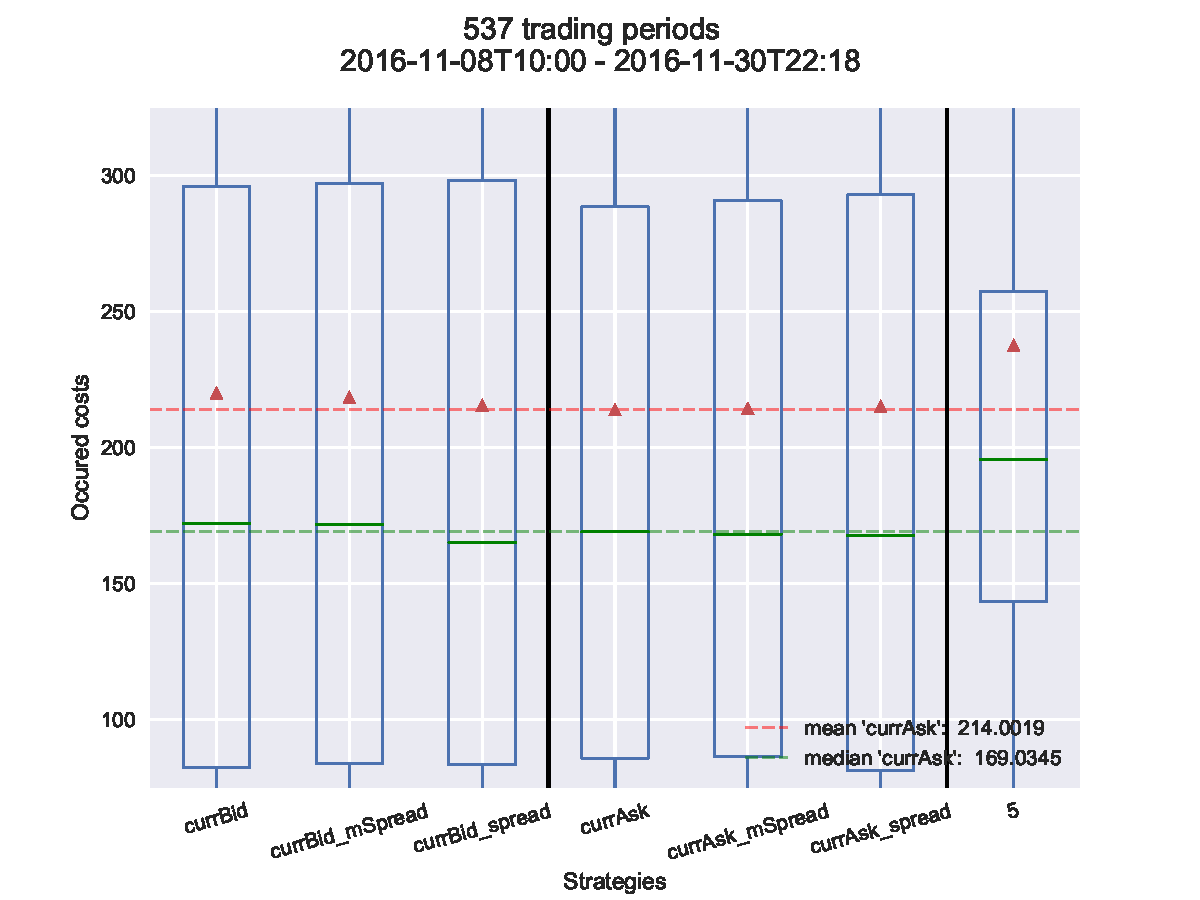
\includegraphics[width=\textwidth]{content/drawings/performance_limitBase_nov}
        		\caption{Slippage.}
		\label{fig:actionlimitmapping:plot}
    	\end{subfigure}%
	\begin{subfigure}[b]{0.40\textwidth}
        		\centering
		\scalebox{0.7}{
\begin{tabular}{lrr}
\toprule
{} &           slippage & performance \\
\midrule
currBid         	     &  220.19 & 92.6\%\\
currBid\_mSpread &  218.71 & 91.9\%\\
currBid\_spread     &  215.76 & 90.7\%\\
\midrule
currAsk                  &  214.00 & 90.0\%\\
currAsk\_mSpread &  214.53 &90.2\%\\
currAsk\_spread    &  215.38 & 90.6\%\\
\midrule
S\&L: 5         	      & 237.75 & 100.0\%\\
MarketOrder          & 737.58 & 310.2\%\\
\bottomrule
\end{tabular}	
		}  \vspace{1.5cm}      		 
        		\caption{Mean slippage.}
		\label{fig:actionlimitmapping:mean}
    	\end{subfigure}

	\caption{Evaluating the impact of different limit base levels.}
	\label{fig:actionlimitmapping}
\end{figure}

In order to produce comparable results, all subsequent experiments are based on the same set of 15 actions: $[-4, -3, ..., 8, 9, 10]$. In line with the formulas presented in \Cref{chap:backwardalgorithm:discussion:actionspace}, these actions translate into order limits deviating by -0.4\% to +1.0\% from the current best price.



\subsection{Baseline}
\label{chap:experiments:baseline}
Simple \ac{SL} strategies (see \Cref{chap:tradingstrategies}) and immediate market order placements serve as benchmark for the performance measurement.\\

Due to bursting Bitcoin prices (see \Cref{fig:ploniexPriceHistory}), the investigated sum of 70.000\$ constitutes a declining contingent of the total market volume. \Cref{fig:runningmean:marketPrice} shows a running average over the amount of slippage, as induced by immediate market orders. Concurrent to declining slippage, the optimal \ac{SL} actions become less aggressive as time passes. The green, dashed lines show the respective average over the train period, which significantly differs from the red, dotted line referring to the average over the test period. \Cref{fig:bestAction} shows the average costs, induced by varying \ac{SL} strategies within the training period.

\begin{figure}[ht]
	\centering
	\begin{subfigure}[b]{0.5\textwidth}
        		\centering
        		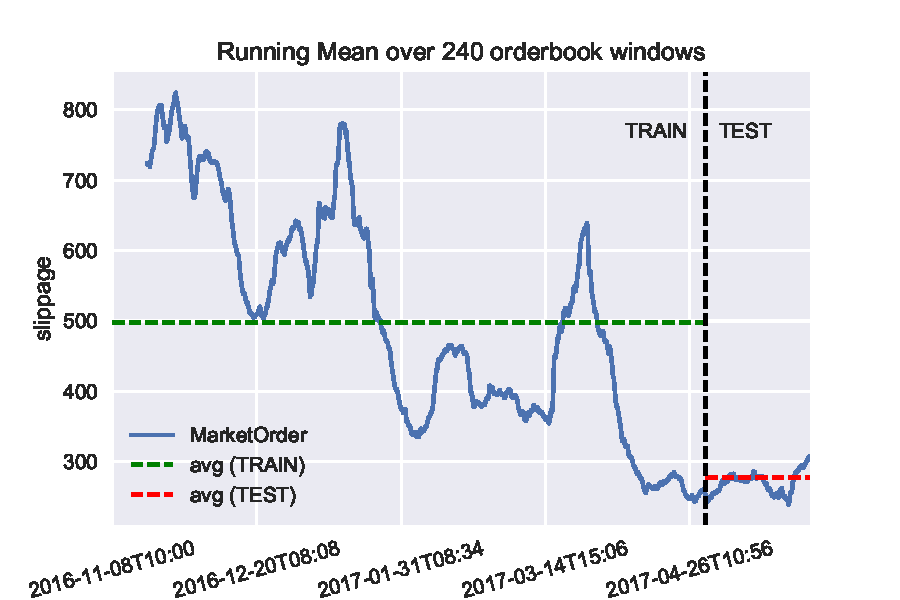
\includegraphics[width=\textwidth]{content/drawings/runningMean240_MarketPrice}
        		\caption{Observed Market Order Slippage.}
		\label{fig:runningmean:marketPrice}
    	\end{subfigure}%
	\begin{subfigure}[b]{0.5\textwidth}
        		\centering
        		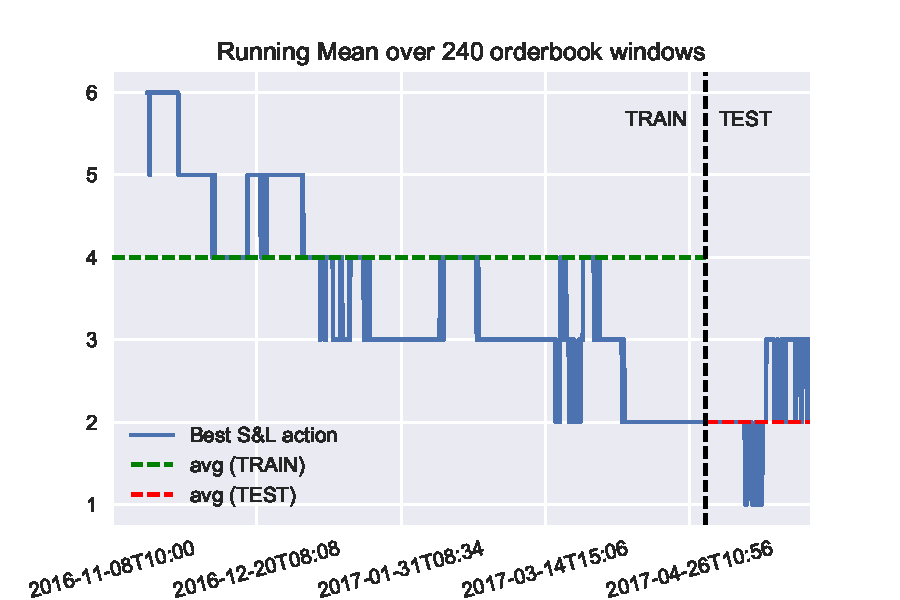
\includegraphics[width=\textwidth]{content/drawings/runningMean240_bestAction}
        		\caption{Best S\&L action.}
		\label{fig:runningmean:bestaction}
    	\end{subfigure}

	\caption{Concurrent to declining slippage, the optimal \ac{SL} actions become less aggressive as time passes.}
	\label{fig:runningmean}
\end{figure}


\begin{figure}[ht]
        	\centering
        	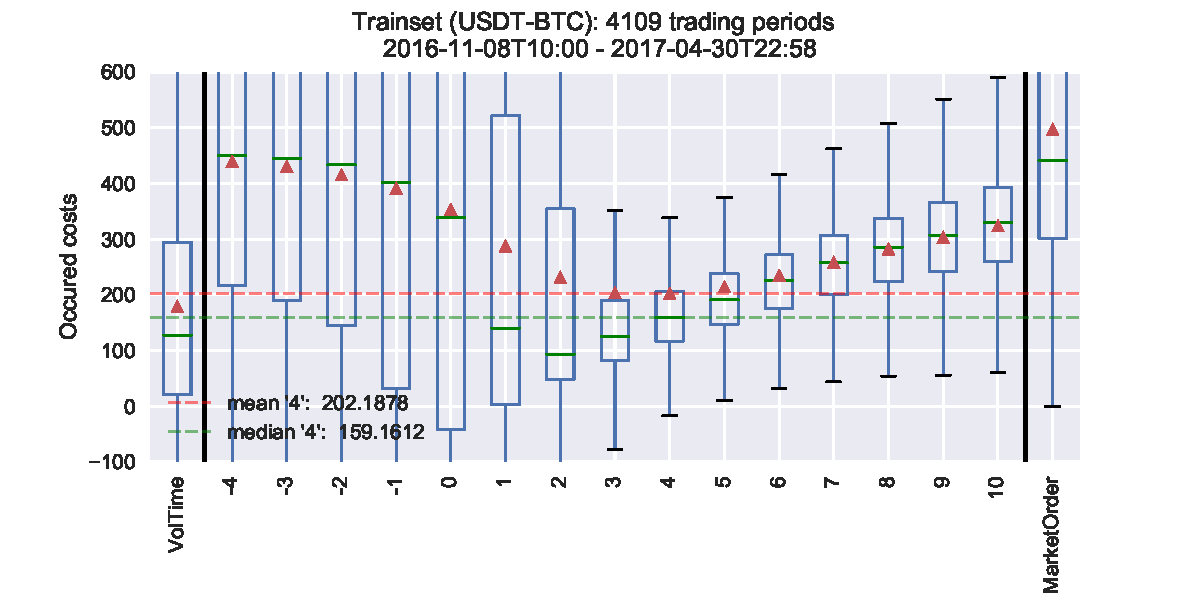
\includegraphics[width=\textwidth]{content/drawings/bestActionTrain}
	\caption{Average costs induced by the varying \ac{SL} actions over the full training period. In average, action 4 performed best.}
	\label{fig:bestAction}
\end{figure}

In order to provide a more realistic and unexaggerated baseline, the optimal \ac{SL} action is estimated from the test period. As such, performance of subsequents experiments are compared to the performance of a simple market order and the \ac{SL} strategy "2", with the initial order limit fixed to 1.002 times the initial ask (\ie $+= 0.2\%$).




\subsection{Additional Market Variables}
\label{chap:exp:additionalmarketvars}
In addition to the market variables proposed in \Cref{chap:actionspace}, the following market level 2 features have been examined: \lstinline!marketPrice_*! describes the relative difference between current center\_price and the worst price that must be paid in case of simple market orders. \lstinline!sharecount_*! quotes the number of Bitcoins, immediately available for 70.000\$.\\

 \Cref{tab:eval:additionalMarketVariables} shows the performance of individual QTable agents trained on private variables plus one discretized market variable attached at a time. While observed trading costs undercut costs induced by simple market orders by -49.14\%, the gain in comparison to the optimal \ac{SL} strategy is far smaller: -10.99\%.\\
 
 Adding the market variable \lstinline!spread! yields a notable improvement of -6.34\% over the plain \lstinline!VolTime!-agent, verifying the findings of Nevmyvaka�\etal \Cite{Nevmyvaka:2006}. However, in contrast to their reported results, the market variable \lstinline!sharecount_buy!, which complies to their \lstinline!Immediate Market Order Cost!, falls flat with a worsening of +6.70\% (compared to -4.26\%).\\

\begin{table}[ht]
	\centering
	
	
	\scalebox{0.6}{
	\begin{tabular}{lrrrllll}
\toprule
{} &  slippage &     med &     std &   perf\_2 &   perf\_4 &   perf\_M & perf\_VolTime \\
\midrule
center\_orig\_disc3            &    149.57 &   46.15 &  420.14 &   94.37\% &   84.81\% &   53.90\% &       99.30\% \\
center\_orig\_disc5            &    161.70 &   37.83 &  450.36 &  102.03\% &   91.68\% &   58.27\% &      107.35\% \\
ImmCost\_buy\_worst\_disc5  &    146.83 &   39.62 &  351.77 &   92.64\% &   83.25\% &   52.92\% &       97.48\% \\
ImmCost\_sell\_worst\_disc5 &    148.94 &   42.71 &  388.86 &   93.97\% &   84.45\% &   53.67\% &       98.88\% \\
ImmCost\_spread\_disc5     &    150.46 &   44.15 &  371.32 &   94.93\% &   85.31\% &   54.22\% &       99.89\% \\
ImmCost\_imbalance\_disc5      &    150.10 &   68.68 &  \cellcolor{green!25}336.60 &   94.71\% &   85.10\% &   54.09\% &       99.65\% \\
sharecount\_buy\_disc3         &    149.57 &   46.15 &  420.14 &   94.37\% &   84.81\% &   53.90\% &       99.30\% \\
sharecount\_buy\_disc5         &    160.73 &   37.78 &  449.22 &  101.41\% &   91.13\% &   57.92\% &      \cellcolor{red!25}106.70\% \\
sharecount\_imbalance\_disc5   &    148.03 &   40.49 &  372.86 &   93.40\% &   83.93\% &   53.35\% &       98.27\% \\
sharecount\_sell\_disc5        &    151.50 &   47.49 &  425.35 &   95.59\% &   85.90\% &   54.60\% &      100.58\% \\
sharecount\_spread\_disc5      &    148.93 &   40.84 &  352.12 &   93.97\% &   84.44\% &   53.67\% &       98.87\% \\
spread\_disc3                 &    147.41 &   35.48 &  370.96 &   93.01\% &   83.58\% &   53.12\% &       97.86\% \\
spread\_disc5                 &    \cellcolor{green!25}141.07 &   \cellcolor{green!25}37.39 &  349.72 &   \cellcolor{green!25}89.01\% &   \cellcolor{green!25}79.98\% &   \cellcolor{green!25}50.84\% &       \cellcolor{green!25}93.66\% \\
spread\_disc9                 &    142.80 &   36.69 &  364.76 &   90.10\% &   80.97\% &   51.46\% &       94.80\% \\
\midrule
ob\_direction\_disc5           &     61.99 &   97.52 &  319.84 &   \cellcolor{black!15}39.11\% &   35.15\% &   22.34\% &       41.16\% \\
future\_center5\_disc5         &    141.61 &   41.79 &  389.58 &   89.35\% &   80.29\% &   51.03\% &       94.02\% \\
future\_center15\_disc5        &    133.78 &   40.90 &  405.88 &   84.41\% &   75.85\% &   48.21\% &       88.82\% \\
future\_center60\_disc5        &    131.85 &   47.63 &  391.46 &   \cellcolor{black!15}83.19\% &   74.75\% &   47.51\% &       87.53\% \\
\midrule
VolTime                      &    150.63 &   \cellcolor{green!25}33.83 &  358.66 &   95.04\% &   85.40\% &   54.28\% &      100.00\% \\
2                            &    158.49 &   69.66 &  400.59 &  100.00\% &   89.86\% &   57.12\% &      105.22\% \\
4                            &    176.37 &  141.66 &  273.58 &  111.28\% &  100.00\% &   63.56\% &      117.09\% \\
MarketOrder                  &    277.49 &  246.48 &  158.66 &  175.08\% &  157.33\% &  100.00\% &      184.22\% \\
\bottomrule
\end{tabular}
	}  		 
        		\caption{An excerpt from the average trading costs within the test period.}
		See \Cref{tab:eval:additionalMarketVariables:fulltable} in the Appendix for complete results.
		\label{tab:eval:additionalMarketVariables}

\end{table}

The exact reason, why individual market variables had such little effect, is unclear, but one possible explanations lies in the data set employed. The original experiment assessed a different data quality. Due to the low resolution of the available orderbook snapshots, a large fraction of the market activity remains inaccessible and consequently the majority of trading opportunities are missed by the agents. Furthermore, the minute time-scaled limit order book data inevitably requires the trading horizon to be rather long. Experiments with shorter time horizons nullified the achievable savings, while longer time horizons led to unacceptable computation times. Consequently, the agents where trained on 4.109 sixty-minute orderbook windows, while Nevmyvaka \etal invoked 45.000 two-minute orderbook windows.


\subsection*{Look-Ahead Features}
\label{chap:experiments:lookahead}
In order to proof the algorithms general ability to find costs reducing order limits, look-ahead features\footnote{look-ahead features provide a glance into the future, and are thus equivalent to cheating.} were added to the universe of market variables. \lstinline!future_center*! quotes percentual changes between the current center price and the center price in 5, 15 and 60 minutes respectively. This hypothetical knowledge about future price trends reduced observed trading costs by -16.81\%.\\

An vastly larger impact (-60.89\%) was observed for the look-ahead feature \lstinline!ob_direction!, quoting the general price trend of the currently observed orderbook window. In contrast to the \lstinline!future_center*! variables, it's value stays constant within individual orderbook windows: \lstinline!orderbook[-1].get_center() / orderbook[0].get_center()!, which seems to provoke more stable strategies.

\subsection*{Discretization Resoution}
\label{chap:experiments:discretization}
While valuable market variables (\ie \lstinline!spread!, \lstinline!ob_direction!, \lstinline!future_center*!) could profit from a larger discretion resolution, this was not the case for the other variables examined.

\subsection*{Constant Market Variables}
\label{chap:exp:additionalmarketvars:constant}
The findings from the look-ahead features encouraged for a supplementary experiment. Rather than considering the actual market situation, the market situation was observed once (at \lstinline!t=0!), and kept frozen for the remaining trading horizon. Hope was, to provoke more stable strategies, as the agents could potentially decide on a \emph{major} strategy and consequently only adapt the limits to the private variables representing the actual trade progress.\\

While \Cref{tab:eval:additionalMarketVariables:fixed} shows improved performance for previous bad performers, the leading \lstinline!spread! dropped from -6.34\% to -4.98\%. Contrary to initial hopes, this approach did not lead to superior performance and was not further persued.
\begin{table}[ht]
	\centering
	
	
	\scalebox{0.6}{
	\begin{tabular}{lrrrllll}
\toprule
{} &  slippage &     med &     std &   perf\_2 &   perf\_4 &   perf\_M & perf\_VolTime \\
\midrule
center\_orig\_disc3            &    149.57 &   46.15 &  420.14 &   94.37\% &   84.81\% &   53.90\% &       99.30\% \\
center\_orig\_disc5            &    150.37 &   47.01 &  422.14 &   94.88\% &   85.26\% &   54.19\% &       \cellcolor{red!25}99.83\% \\
ImmCost\_buy\_worst\_disc5  &    150.22 &   50.15 &  402.48 &   94.78\% &   85.17\% &   54.13\% &       99.73\% \\
ImmCost\_sell\_worst\_disc5 &    157.24 &   42.71 &  378.90 &   99.21\% &   89.15\% &   56.67\% &      104.39\% \\
ImmCost\_spread\_disc5     &    151.25 &   53.07 &  397.30 &   95.43\% &   85.75\% &   54.51\% &      100.41\% \\
ImmCost\_imbalance\_disc5      &    147.26 &   47.03 &  383.23 &   92.91\% &   83.49\% &   53.07\% &       \cellcolor{black!15}97.76\% \\
sharecount\_buy\_disc3         &    149.57 &   46.15 &  420.14 &   94.37\% &   84.81\% &   53.90\% &       99.30\% \\
sharecount\_buy\_disc5         &    150.37 &   47.01 &  422.14 &   94.88\% &   85.26\% &   54.19\% &       \cellcolor{red!25}99.83\% \\
sharecount\_imbalance\_disc5   &    152.44 &   53.41 &  400.89 &   96.18\% &   86.43\% &   54.94\% &      101.21\% \\
sharecount\_sell\_disc5        &    150.37 &   47.01 &  422.14 &   94.88\% &   85.26\% &   54.19\% &       99.83\% \\
sharecount\_spread\_disc5      &    149.23 &   53.41 &  402.65 &   94.16\% &   84.61\% &   53.78\% &       99.07\% \\
spread\_disc3                 &    148.83 &   41.70 &  360.98 &   93.91\% &   84.39\% &   53.64\% &       98.81\% \\
spread\_disc5                 &    \cellcolor{green!25}143.12 &   \cellcolor{green!25}40.78 &  \cellcolor{green!25}350.14 &   \cellcolor{green!25}90.30\% &   \cellcolor{green!25}81.15\% &   \cellcolor{green!25}51.58\% &       \cellcolor{green!25}95.02\% \\
spread\_disc9                 &    144.66 &   43.25 &  352.39 &   91.27\% &   82.02\% &   52.13\% &       96.04\% \\
\midrule
ob\_direction\_disc5           &     61.99 &   97.52 &  319.84 &   39.11\% &   35.15\% &   22.34\% &       41.16\% \\
\midrule
VolTime                      &    150.63 &   33.83 &  358.66 &   95.04\% &   85.40\% &   54.28\% &      100.00\% \\
2                            &    158.49 &   69.66 &  400.59 &  100.00\% &   89.86\% &   57.12\% &      105.22\% \\
4                            &    176.37 &  141.66 &  273.58 &  111.28\% &  100.00\% &   63.56\% &      117.09\% \\
MarketOrder                  &    277.49 &  246.48 &  158.66 &  175.08\% &  157.33\% &  100.00\% &      184.22\% \\
\bottomrule
\end{tabular}
	}  		 
        		\caption{An excerpt from the average trading costs within the test period.}
		In contrast to \Cref{tab:eval:additionalMarketVariables}, market variables originate from the very first orderbook of the respective orderbook window.
		See \Cref{tab:eval:additionalMarketVariables:fixed:fulltable} in the Appendix for complete results.
		\label{tab:eval:additionalMarketVariables:fixed}

\end{table}



\subsection{Cost function}
default: slippage based on initial\_center

experimental: Improvement over MarketPrice





\subsection*{Function Approximation}
\begin{itemize}
\item RandomForest (BatchTree Agent)
\item NN Agent
\end{itemize}



\subsection{Forward Sampling}
\begin{itemize}
\item Growing batch learning
\item Experience Replay (NN\_Agent)
\item Exploration vs avoidance of repeatedly trying same actions.
\item Markov Property violated
\item Realistic samples, no rounding. Better fit for \emph{curious} masterbook shapes as described in \Cref{chap:modelcorrectness}?!
\end{itemize}














\cleardoublepage{}